\chapter{Implementatie}

\label{Chapter6}

Dit hoofdstuk gaat over de deelvraag \enquote{\deelimplementatie}

\section{Feature-environments}
Nieuwe infrastructuur:
\begin{figure}[h]
	\centering
	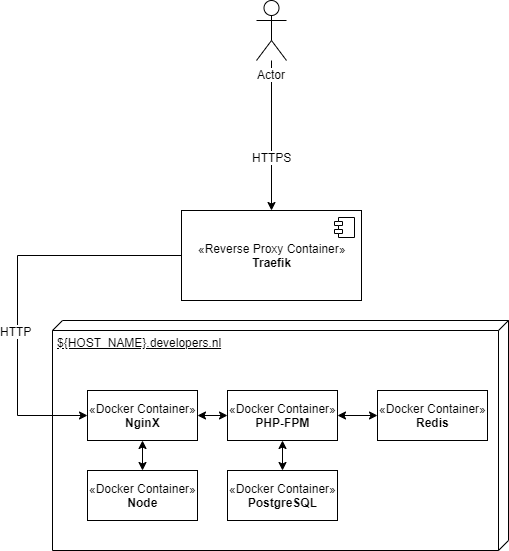
\includegraphics[width=13cm]{Figures/Traefik}
	\decoRule
	\caption[Traefik Infrastructure]{Nieuwe infrastructuur met Traefik reverse proxy}
	\label{fig:traefikinfrastructure}
\end{figure}
\\Activity Diagram:
\begin{figure}[h]
	\centering
	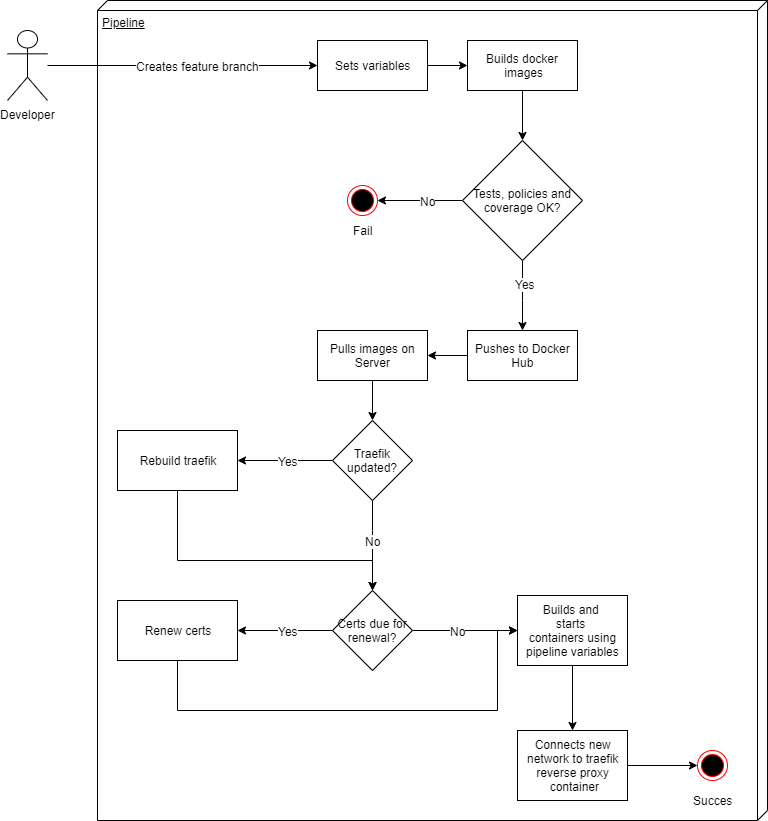
\includegraphics[width=13cm]{Figures/Activitydiagram}
	\decoRule
	\caption[Pipeline Activity Diagram]{Activity Diagram voor de pipeline}
	\label{fig:activitydiagram}
\end{figure}

\section{Codecov}
Code voor het implementeren is te zien in bijlage \ref{codecov}

\section{Opschonen Docker volumes en images}
\texttt{developers.nl/ansible/group\_vars/all.yml}
\begin{minted}[linenos=true, bgcolor=codebg]{yaml}
image_delete_until_time: 4h
\end{minted}
\texttt{developers.nl/ansible/deploy.yml}
\begin{minted}[linenos=true, bgcolor=codebg]{yaml}
- name: "Clean up images older than {{ image_delete_until_time }}"
  docker_prune:
    images: yes
    images_filters:
      dangling: false
      until: "{{ image_delete_until_time }}"
  register: prune_result
\end{minted}
